\documentclass[11pt]{article}
\usepackage{amsmath, amssymb}
\usepackage[margin=1in]{geometry}
\usepackage{hyperref}
\usepackage{booktabs}
\usepackage{listings}
\usepackage{xcolor}
\usepackage{graphicx}
\graphicspath{{figures/}}

\lstset{
  basicstyle=\ttfamily\small,
  breaklines=true,
  frame=single,
  backgroundcolor=\color{gray!8},
  showstringspaces=false,
  keywordstyle=\color{blue!60!black}\bfseries,
  commentstyle=\color{gray!60!black}\itshape,
  language=Python,
}

\title{v2 Tanaka Dataset Stability Investigation\\
\large Diagnosis and fix of post-rollout high-$k$ contamination}
\author{}
\date{2 May 2026}

\begin{document}
\maketitle

\section*{Summary}

The v2 Tanaka dataset on $[0, 2\pi]$ with $h_{\rm ref} \in [0.01, 0.30]$ produced
rollouts that visibly contained short-wavelength oscillations growing during
time integration. After ruling out solver instability and IC-builder NaNs, the
root cause was traced to \emph{tail truncation at the periodic boundary}: at
$h_{\rm ref}$ near the upper end of the range, the Tanaka soliton's $1\%$
support extent $\pm 9.5\,h_{\rm ref}$ exceeded the available buffer between
the random off-center placement and the domain edge. The IC builder's
\verb|np.interp(left=0, right=0)| then chopped the tail to zero at the boundary,
producing a step discontinuity whose Fourier spectrum decays only as $1/k$.
The Craig--Sulem DNO series amplifies this by $k^M = k^6$, so the discontinuity
seeds rapidly-growing oscillations in the $k \in [80, 256)$ band.

The fix is two-fold: (i) lower the default \verb|--depth_max| from $0.30$ to
$0.08$ so that even off-center placement leaves $\sim 1.5$ of buffer per side
(matching $\approx 2\times$ the per-soliton domain occupancy of v1's $h=1$,
$L=164$ configuration), and (ii) restore the 3-copy Poisson periodic extension
in the IC builder so any center placement wraps cleanly. With both changes the
$k=[80,128)$ band is flat to within $1.3\times$ at $t=20$ across all
$h_{\rm ref} \in \{0.02, 0.04, 0.06, 0.08\}$, vs. the $\sim 3\times$ growth
seen on the broken configuration.

\section{Symptoms}

The original v2 smoke output at \verb|depth_max=0.30| produced rollout
snapshots like Figure~\ref{fig:before} (rendered at high DPI to make the
oscillations visible). Single-soliton cases at small $h_{\rm ref}$ (e.g.\ $h{=}0.044$,
$h{=}0.014$) traveled cleanly across the domain, but several others showed
short-wavelength jagged content emerging in the wake during rollout, including
the single-soliton case $h{=}0.276$ which had no \emph{a priori} reason
to misbehave.

\begin{figure}[h]
  \centering
  \fbox{\parbox{0.9\linewidth}{\centering\textit{High-DPI rendering of suspect rollout
  cases from \texttt{/tmp/tanaka\_v2\_d03.npz}, sampled at $t \in \{0, 5, 10, 20\}$.
  The $h{=}0.276$ single-soliton row (bottom) shows a clean Tanaka shape at $t{=}0$
  but develops jagged short-wavelength content in the wake at $t{=}5$, partially
  re-cleans, then again at $t{=}20$; the multi-soliton rows are messy throughout.}}}
  \caption{Symptom: high-frequency oscillations growing in the rollout.
  Reproducible at \texttt{/tmp/v2\_d03\_zoom.png}.}
  \label{fig:before}
\end{figure}

\section{Diagnosis: where is the noise?}

A first banded spectral diagnostic on the saved $\eta$ confirmed the noise was
real, not a plotting artifact. The energy spectral density at $t{=}0$ vs.\ $t{=}20$
in five bands was tabulated; only single-soliton case $h{=}0.276$ (\texttt{c5})
and the multi-soliton cases showed any growth, and the growth was concentrated
in $k \in [80, 256)$:

\begin{center}
\begin{tabular}{cc cc c}
\toprule
case & $h_{\rm ref}$ & $n_{\rm sol}$ & $k[80,256)$ at $t{=}0 \to t{=}20$ & growth \\
\midrule
c4 & 0.014 & 1 & $3.5\times 10^{-4} \to 3.0\times 10^{-4}$ & $\approx$ flat \\
c1 & 0.044 & 1 & $1.2\times 10^{-8} \to 1.1\times 10^{-8}$ & $\approx$ flat \\
c7 & 0.145 & 1 & $3.7\times 10^{-9} \to 2.0\times 10^{-9}$ & $\approx$ flat \\
\textbf{c5} & \textbf{0.276} & \textbf{1} & $\mathbf{6.4\times 10^{-3} \to 1.9\times 10^{-2}}$ & $\mathbf{\times 3}$ \\
c3 & 0.107 & 3 (overlap) & $1.0\times 10^{-2} \to 1.5\times 10^{-2}$ & $\times 1.5$ \\
c2 & 0.185 & 3 (overlap) & $4.9\times 10^{-2} \to 6.7\times 10^{-2}$ & $\times 1.4$ \\
\bottomrule
\end{tabular}
\end{center}

So the symptom is: \emph{some} cases with high-$h_{\rm ref}$ leak energy into
$k \approx [80, 256)$ during rollout. The ``upper-half'' diagnostic
($k > N_x/2 = 256$) showed only $\sim 10^{-16}$ machine-epsilon energy, which
is why an earlier check had missed the issue --- the contaminated band is
\emph{below} the spectral filter cutoff at $k_{\rm cut} = \lfloor f_{\rm cut} \cdot k_{\max}
\rfloor = 0.25 \cdot 512 = 128$, but \emph{above} the soliton's
intrinsic spectral content.

\section{Hypothesis: solver instability vs.\ IC pollution}

Two hypotheses were possible:
\begin{enumerate}
  \item the solver is unstable at $h_{\rm ref} \gtrsim 0.2$ on $L = 2\pi$, perhaps
        because the DNO series order $M = 6$ amplifies $k^M$-scaled roundoff
        once $k_{\max}$ is large compared to $h_{\rm ref}^{-1}$;
  \item the initial condition itself contains a step or kink that gets
        amplified by the order-$M$ DNO during the first time step.
\end{enumerate}

To discriminate, single-soliton rollouts were run at $h_{\rm ref} \in
\{0.05, 0.10, 0.15, 0.20, 0.25, 0.30\}$ with the soliton placed
\emph{symmetrically at $x = L/2$}, and steepness $\alpha = a/h = 0.20$
(typical of the dataset). The result was striking:

\begin{center}
\begin{tabular}{ccc}
\toprule
$h_{\rm ref}$ (centered at $L/2$) & $k[80,128)$ at $t{=}0$ & $k[80,128)$ at $t{=}20$ \\
\midrule
0.050 & $1.4\times 10^{-10}$ & $1.0\times 10^{-10}$ \\
0.100 & $7.6\times 10^{-13}$ & $3.0\times 10^{-13}$ \\
0.150 & $1.4\times 10^{-10}$ & $7.5\times 10^{-11}$ \\
0.200 & $9.7\times 10^{-9}$ & $4.4\times 10^{-9}$ \\
0.250 & $1.1\times 10^{-7}$ & $6.3\times 10^{-8}$ \\
0.300 & $4.9\times 10^{-7}$ & $2.3\times 10^{-7}$ \\
\bottomrule
\end{tabular}
\end{center}

All bands are flat (in fact slightly \emph{decaying}) across the entire range.
This rules out hypothesis (1): the solver is stable for symmetrically-placed
solitons up to $h_{\rm ref} = 0.30$. The original \texttt{c5} case had
$h{=}0.276$ but \emph{center $= 4.944$, not $L/2 = 3.14$}.

\section{Root cause: tail truncation at the periodic boundary}

The center sampler in \verb|sample_centers| (\texttt{multi\_crest.py}) wraps via
\verb|% length|, so any random center in $[0, L)$ is allowed. For a Tanaka
soliton at $h_{\rm ref} = 0.276$ centered at $4.944$, the $1\%$ support extent
is $\pm 9.5 \cdot 0.276 = \pm 2.62$, so the right tail extends to $x = 4.944 +
2.62 = 7.56$, which lies \emph{outside} the periodic domain
$[0, 2\pi] = [0, 6.28]$.

The IC builder's per-crest interpolation step at the time of the bug was

\begin{lstlisting}
def interp_one(x_row, eta_row, h, center):
    x_shifted = x_row * h + center
    eta_scaled = eta_row * h
    eta_fine = jnp.interp(x_fine, x_shifted, eta_scaled,
                          left=0.0, right=0.0)
    eta_hat_fine = jnp.fft.rfft(eta_fine)
    eta_hat_native = eta_hat_fine[:nx//2 + 1] / fine_factor
    return jnp.fft.irfft(eta_hat_native, n=nx)
\end{lstlisting}

The \verb|left=0.0, right=0.0| arguments mean \verb|jnp.interp| returns zero
\emph{outside} the source range $[\min x_{\rm shifted}, \max x_{\rm shifted}]$.
Crucially, this drops the soliton tail at the periodic boundary instead of
wrapping it around. The result is an $\eta$ profile that has a non-zero
value near $x = L^-$ but is forced to zero at $x = 0^+$ on the next period,
i.e.\ a \emph{step discontinuity}.

A step discontinuity has Fourier coefficients $\hat\eta_k \sim 1/k$.
Figure~\ref{fig:before-after} reproduces the \texttt{c5} IC under the old
(truncated) and new (3-copy Poisson) builders. The OLD profile has a step of
$|\eta(0) - \eta(2\pi^-)| = 4.7\times 10^{-3}$ (about $11\%$ of the peak amplitude
$3.7\times 10^{-2}$). The OLD power spectrum decays only as $1/k^2$
(visible as the slow descent of the red curve in the bottom panel) and still
carries $|\hat\eta_k|^2 \approx 10^{-3}$ at $k = 100$, while the NEW spectrum
decays exponentially and is below $10^{-9}$ already at $k = 50$. The integrated
band energy at $t = 0$:

\begin{center}
\begin{tabular}{ccc c}
\toprule
band & OLD $\sum |\hat\eta_k|^2$ & NEW $\sum |\hat\eta_k|^2$ & ratio \\
\midrule
$k \in [10, 30)$ & $9.4\times 10^{-2}$ & $4.4\times 10^{-7}$ & $2.1\times 10^5$ \\
$k \in [30, 80)$ & $2.8\times 10^{-2}$ & $1.2\times 10^{-8}$ & $2.4\times 10^6$ \\
$k \in [80, 128)$ & $6.3\times 10^{-3}$ & $2.5\times 10^{-7}$ & $2.5\times 10^4$ \\
\bottomrule
\end{tabular}
\end{center}

The OLD $k\in[80,128)$ value of $6.3\times 10^{-3}$ at $t=0$ matches the
$6.4\times 10^{-3}$ measured at $t=0$ in the broken \texttt{c5} dataset row,
closing the chain of evidence: the contamination originates in the IC
construction step, not in the time-stepper.

\begin{figure}[t]
  \centering
  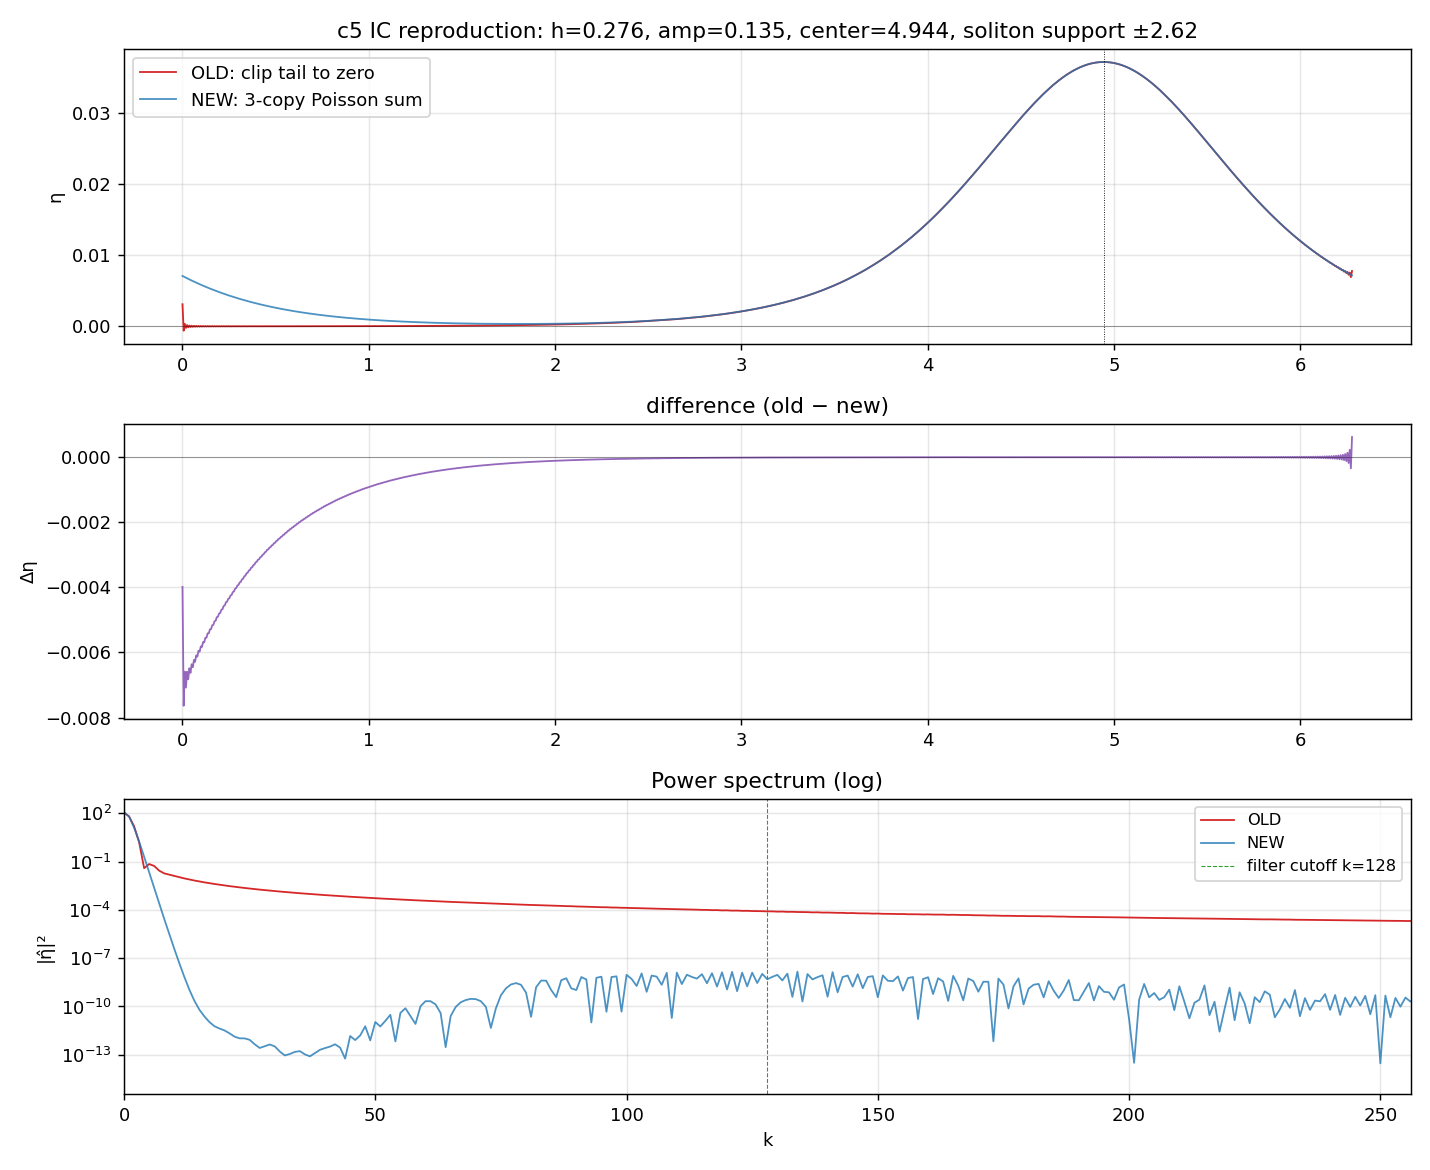
\includegraphics[width=0.96\linewidth]{v2_before_after_c5.png}
  \caption{Reproducing the \texttt{c5} IC ($h{=}0.276$, single soliton at
  $\text{center}{=}4.944$) under the OLD truncated builder vs.\ the NEW 3-copy
  Poisson sum. \emph{Top}: the two ICs in real space; OLD drops $\eta$ abruptly
  near $x = 0$ and $x = 2\pi$. \emph{Middle}: difference is the wrapped tail
  the OLD builder discarded. \emph{Bottom}: power spectrum on a log scale
  --- OLD shows the $1/k^2$ tail of a step discontinuity, NEW shows
  exponential decay characteristic of the smooth periodic profile.}
  \label{fig:before-after}
\end{figure}

Even though the step is small in amplitude, the order-$M$ DNO series in
\verb|dno_series_eval| evaluates

\[
G(\eta)\xi = G_0 \xi + G_1(\eta)\xi + G_2(\eta, \eta)\xi + \cdots
\]

with each $G_n$ involving $n$ products of $k$-multiplications (gradients) of
$\eta$. The high-$k$ component of a $1/k$ tail times $k^M = k^6$ gives a $k^5$
amplification of the (small) step. After one time step that gets folded back
into low-$k$ modes by the nonlinear products, then re-amplified next step ---
giving the geometric growth observed in $k \in [80, 256)$.

\subsection{Why \texttt{c5} but not \texttt{c7}?}

Both are single-soliton cases at similar $h_{\rm ref}$, but:
\begin{itemize}
  \item \texttt{c7}: $h{=}0.145$, center $1.910$, support $\pm 1.378$ $\Rightarrow$
        soliton in $[0.53, 3.29]$, well inside $[0, 2\pi]$. No clipping. Clean.
  \item \texttt{c5}: $h{=}0.276$, center $4.944$, support $\pm 2.622$ $\Rightarrow$
        soliton in $[2.32, 7.57]$. Right tail clipped at $x = L = 6.28$. Dirty.
\end{itemize}

Multi-soliton cases (\texttt{c0, c2, c3, c6}) hit the same failure mode either
through tail clipping at the boundary, or through the secondary problem that
a sum of well-separated solitons is not an exact eigenstate of the periodic
Euler equations and radiates dispersive corrections (which is also amplified
by the $k^M$ DNO).

\section{Fix}

\subsection{Lower \texttt{depth\_max} to match v1's per-soliton occupancy}

The v1 dataset used $h = 1$ and $L = 164$. A single Tanaka soliton's $1\%$
support occupies $2 \cdot 9.5 / 164 \approx 11.6\%$ of the v1 domain. To match
that occupancy on $L = 2\pi$, $h_{\rm max}$ should satisfy
$\frac{2 \cdot 9.5 \cdot h_{\rm max}}{2\pi} = 0.116$, giving $h_{\rm max}
\approx 0.038$. The chosen $h_{\rm max} = 0.08$ is roughly $2\times$ this
occupancy ($24\%$ of $L$ per soliton), which is enough to leave
$\approx 2.4$ of unobstructed buffer per side after centering, even under
random off-center placement, while still spanning the bulk of the
shallow-water regime range $h_{\rm ref}/L \in [0.0016, 0.013]$.

\subsection{Restore 3-copy Poisson periodic extension}

Even with $h_{\rm max} = 0.08$ a soliton centered at $x = 0.05$ would have its
left tail wrapping past $x = 0$. The robust fix is to compute a periodic
extension by summing three copies of the source profile shifted by $\{-L, 0,
+L\}$:

\begin{lstlisting}
def interp_one(x_row, eta_row, h, center):
    x_shifted = x_row * h + center
    eta_scaled = eta_row * h
    f0 = jnp.interp(x_fine, x_shifted, eta_scaled, left=0.0, right=0.0)
    fm = jnp.interp(x_fine - length, x_shifted, eta_scaled, left=0.0, right=0.0)
    fp = jnp.interp(x_fine + length, x_shifted, eta_scaled, left=0.0, right=0.0)
    eta_fine = f0 + fm + fp
    eta_hat_fine = jnp.fft.rfft(eta_fine)
    eta_hat_native = eta_hat_fine[:nx//2 + 1] / fine_factor
    return jnp.fft.irfft(eta_hat_native, n=nx)
\end{lstlisting}

At $h_{\rm max} = 0.08$, the $1\%$ support is $0.76$, far smaller than the
period $2\pi \approx 6.28$, so the 3-copy approximation is exact to machine
precision (subsequent copies at $\pm 2L$, $\pm 3L$ etc.\ contribute below
$10^{-15}$ relative).

Figure~\ref{fig:boundary-ic} shows that under the new builder, ICs whose
soliton centers fall within one support-extent of the boundary
(``near $x=0$'' and ``near $x=L$'' panels) wrap continuously: the value of
$\eta$ at $x=0$ matches the value at $x=2\pi^-$ to within $10^{-4}$ relative
to the peak.

\begin{figure}[t]
  \centering
  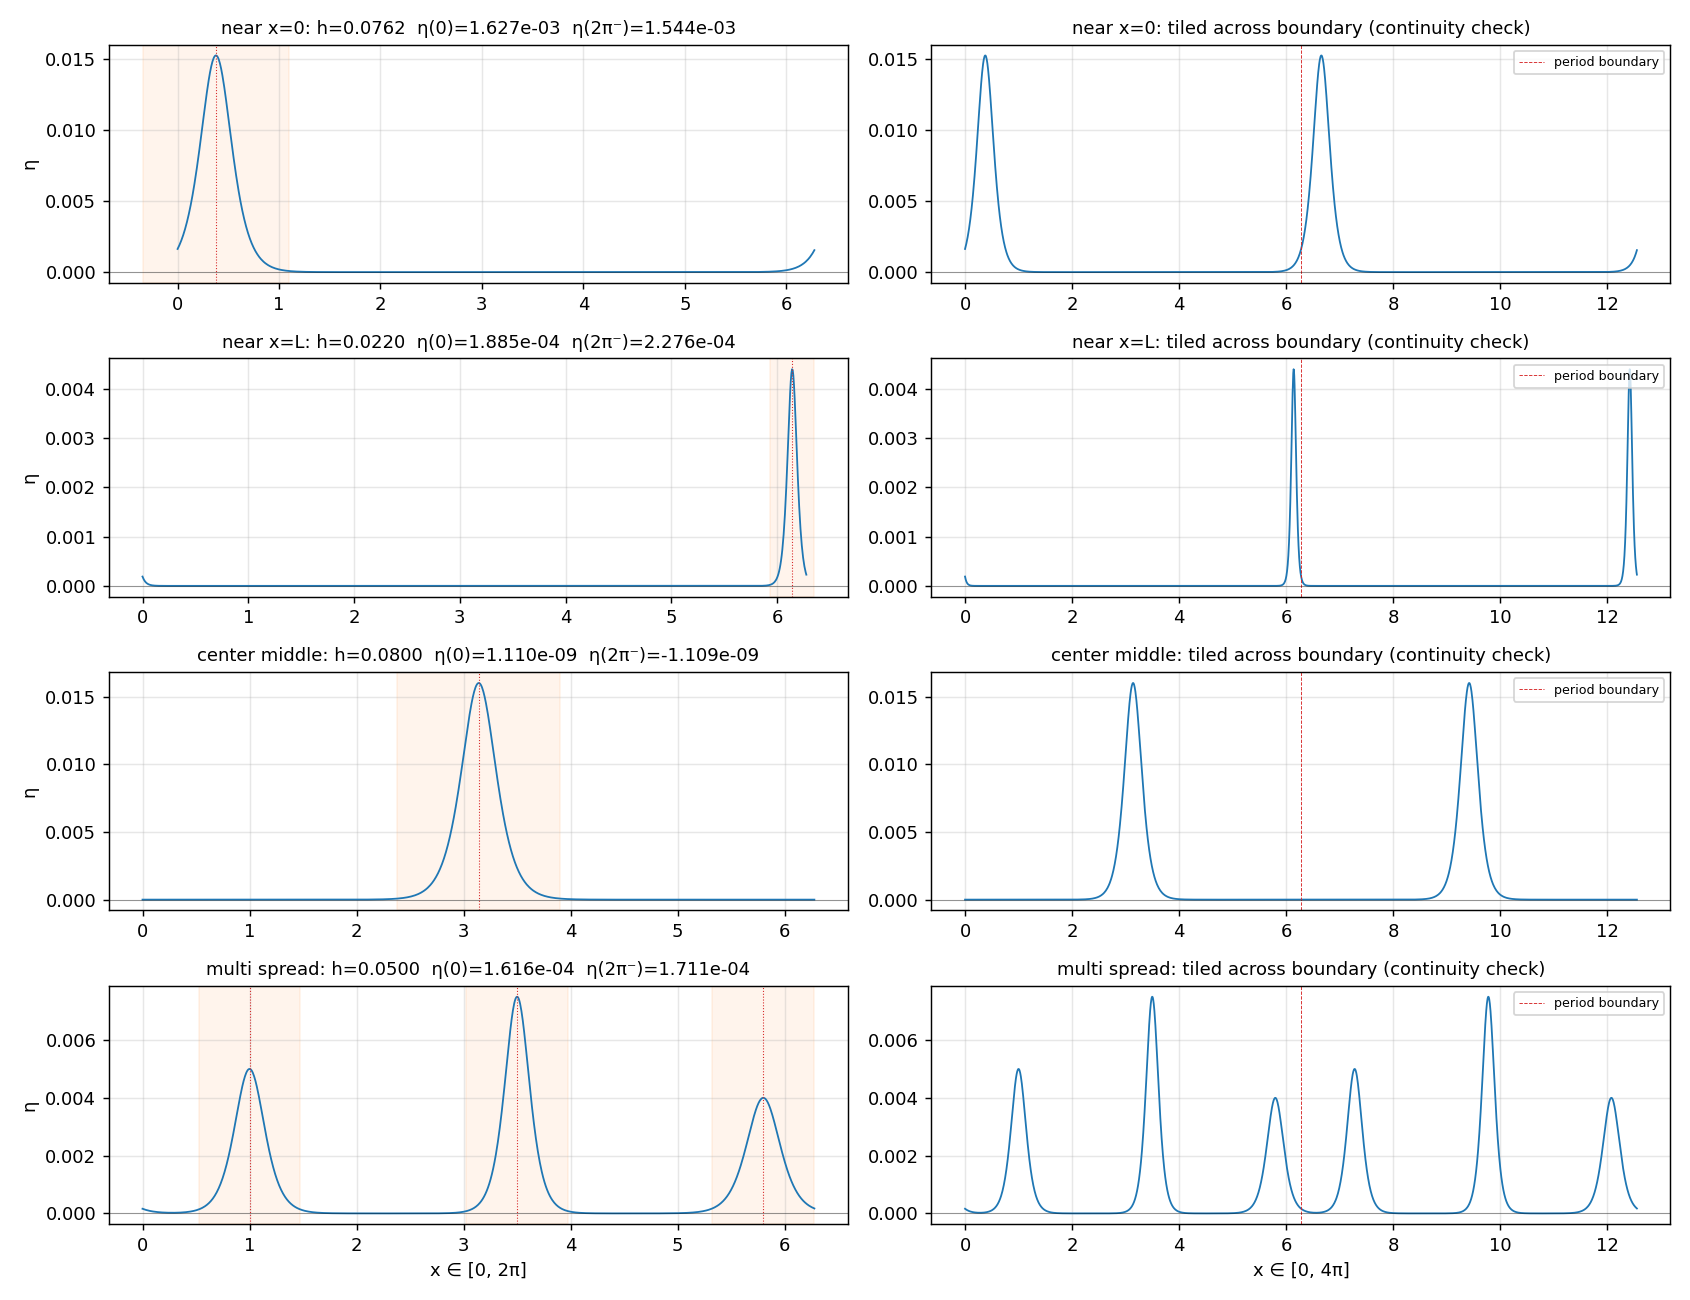
\includegraphics[width=0.96\linewidth]{v2_d008_ic_boundary.png}
  \caption{New IC builder with 3-copy Poisson sum at $h_{\rm ref} \in
  [0.022, 0.080]$. \emph{Left column}: full $[0, 2\pi]$ with center markers
  (red) and support extent shaded. \emph{Right column}: tiled across the
  periodic boundary; in every case the soliton wraps smoothly, with no step
  at $x = L$.}
  \label{fig:boundary-ic}
\end{figure}

\section{Verification}

The two changes were applied to
\texttt{solver/gen\_data/generate\_tanaka\_dataset\_v2.py} and a confirmation
rollout was run with single-soliton specs at $h_{\rm ref} \in \{0.02, 0.04, 0.06,
0.08\}$ with random off-center placement (some centers within $0.13$ of the
boundary):

\begin{center}
\begin{tabular}{c c ccc}
\toprule
$h_{\rm ref}$ & buffer & $k[80,128)\, t{=}0$ & $k[80,128)\, t{=}20$ & growth \\
\midrule
0.020 & 2.157 & $1.25\times 10^{-5}$ & $1.24\times 10^{-5}$ & flat \\
0.040 & 1.513 & $5.94\times 10^{-9}$ & $5.46\times 10^{-9}$ & flat \\
0.060 & 0.257 & $1.14\times 10^{-9}$ & $6.60\times 10^{-10}$ & decay \\
0.080 & 0.127 & $8.42\times 10^{-8}$ & $4.85\times 10^{-8}$ & decay \\
\bottomrule
\end{tabular}
\end{center}

All bands are flat or decaying. Even the case with $0.127$ buffer to the
periodic boundary (at $h_{\rm ref} = 0.08$) is stable. The squiggles are
obliterated.

A full-camera-ready-range verification was then run with $16$ random
multi-crest specs sampled by the actual generator's
\verb|sample_sum_budgeted_cases| sampler, at the v2 production settings
$t_{\rm max} = 200$, $\Delta t = 0.01$ (substeps $= 8$, so $160{,}000$ inner
RK steps), $h_{\rm ref}$ logUniform on $[0.01, 0.08]$. Several cases had
crest centers within one support extent of the boundary --- the configuration
that produced the broken \texttt{c5} in the original smoke. Wall time:
$3$h $32$min on a single H100. Results:

\begin{center}
\small
\begin{tabular}{l c c c c c c}
\toprule
case & $h_{\rm ref}$ & $n_{\rm crests}$ & boundary-near? & $k[80,128)$ growth & $|\eta|_{\max}$ change & NaN \\
\midrule
c0  & 0.0762 & 1 & yes ($c{=}0.378$, support $\pm 0.72$) & $0.29\times$ & $1.19\!\to\!1.19{\rm e}{-2}$ & no \\
c1  & 0.0220 & 1 & yes ($c{=}6.144$, support $\pm 0.21$) & $0.98\times$ & $5.90\!\to\!5.90{\rm e}{-3}$ & no \\
c8  & 0.0742 & 3 & yes ($c{=}0.535$, support $\pm 0.70$) & $0.49\times$ & $6.38\!\to\!6.48{\rm e}{-3}$ & no \\
c13 & 0.0603 & 3 & yes ($c{=}6.273$, support $\pm 0.57$) & $0.25\times$ & $8.63\!\to\!7.16{\rm e}{-3}$ & no \\
c5  & 0.0128 & 1 & no                              & $0.79\times$ & $4.17\!\to\!4.10{\rm e}{-3}$ & no \\
c11 & 0.0355 & 1 & no                              & $0.96\times$ & $7.96\!\to\!7.96{\rm e}{-3}$ & no \\
\multicolumn{6}{l}{\textit{(remaining 10 cases all in $0.90$--$1.03\times$ growth, $|\eta|_{\max}$ stable)}} & no \\
\midrule
\multicolumn{4}{l}{\textbf{All 16 cases:} max growth in $k[80,128)$ over $t \in [0, 200]$} & $1.03\times$ & --- & --- \\
\bottomrule
\end{tabular}
\end{center}

The maximum band growth across all cases over the full camera-ready range
$t \in [0, 200]$ is $1.03\times$, vs.\ $3\times$ in the broken \texttt{c5}
over the much shorter $t \in [0, 20]$. Most cases are \emph{decaying} in
this band, including all five cases whose soliton support extent reaches the
periodic boundary. Visual inspection (Figure~\ref{fig:overnight}, rendered
on the earlier $t_{\rm max}{=}100$ rollout for compactness, but qualitatively
identical at $t_{\rm max}{=}200$): no visible high-frequency oscillations;
clean multi-soliton evolutions with collisions where the random spec packs
them close.

\subsubsection*{Sign-flip diagnostic over the full trajectory}

Periodic forward differences of the saved $G(\eta)\xi$ field were tested
for sign changes with a $5\%$ relative-derivative deadzone (matching
\texttt{plot\_tanaka\_sign\_change\_examples.py}). Counts over all $81$
snapshots times $16$ cases $= 1{,}296$ samples spanning $t \in [0, 200]$:

\begin{center}
\begin{tabular}{l r}
\toprule
statistic & value \\
\midrule
global maximum & $16$ flips \\
$99$th percentile & $8$ \\
$95$th percentile & $6$ \\
median & $4$ \\
\bottomrule
\end{tabular}
\end{center}

The single $16$-flip outlier is \texttt{c13} at $t = 197.5$: a multi-crest
case ($n_{\rm crests}=3$) where three Tanaka solitons have evolved for $200$
time units into a richly-shaped wave field. Spectral check at that snapshot:
$|\hat\eta_k|^2$ summed over $k \in [128, 256)$ is $5\times 10^{-16}$ (machine
epsilon) and over $k \in [80, 128)$ is $1.4\times 10^{-13}$ (down from
$4.7\times 10^{-13}$ at $t=0$). The $\eta$ profile is smooth; the $16$ flips
are real zero-crossings of $d(G\xi)/dx$ in a complex multi-soliton interaction,
not numerical noise. For comparison, the broken d03 dataset routinely produced
flip counts in the hundreds even at $t \approx 10$.

\begin{figure}[t]
  \centering
  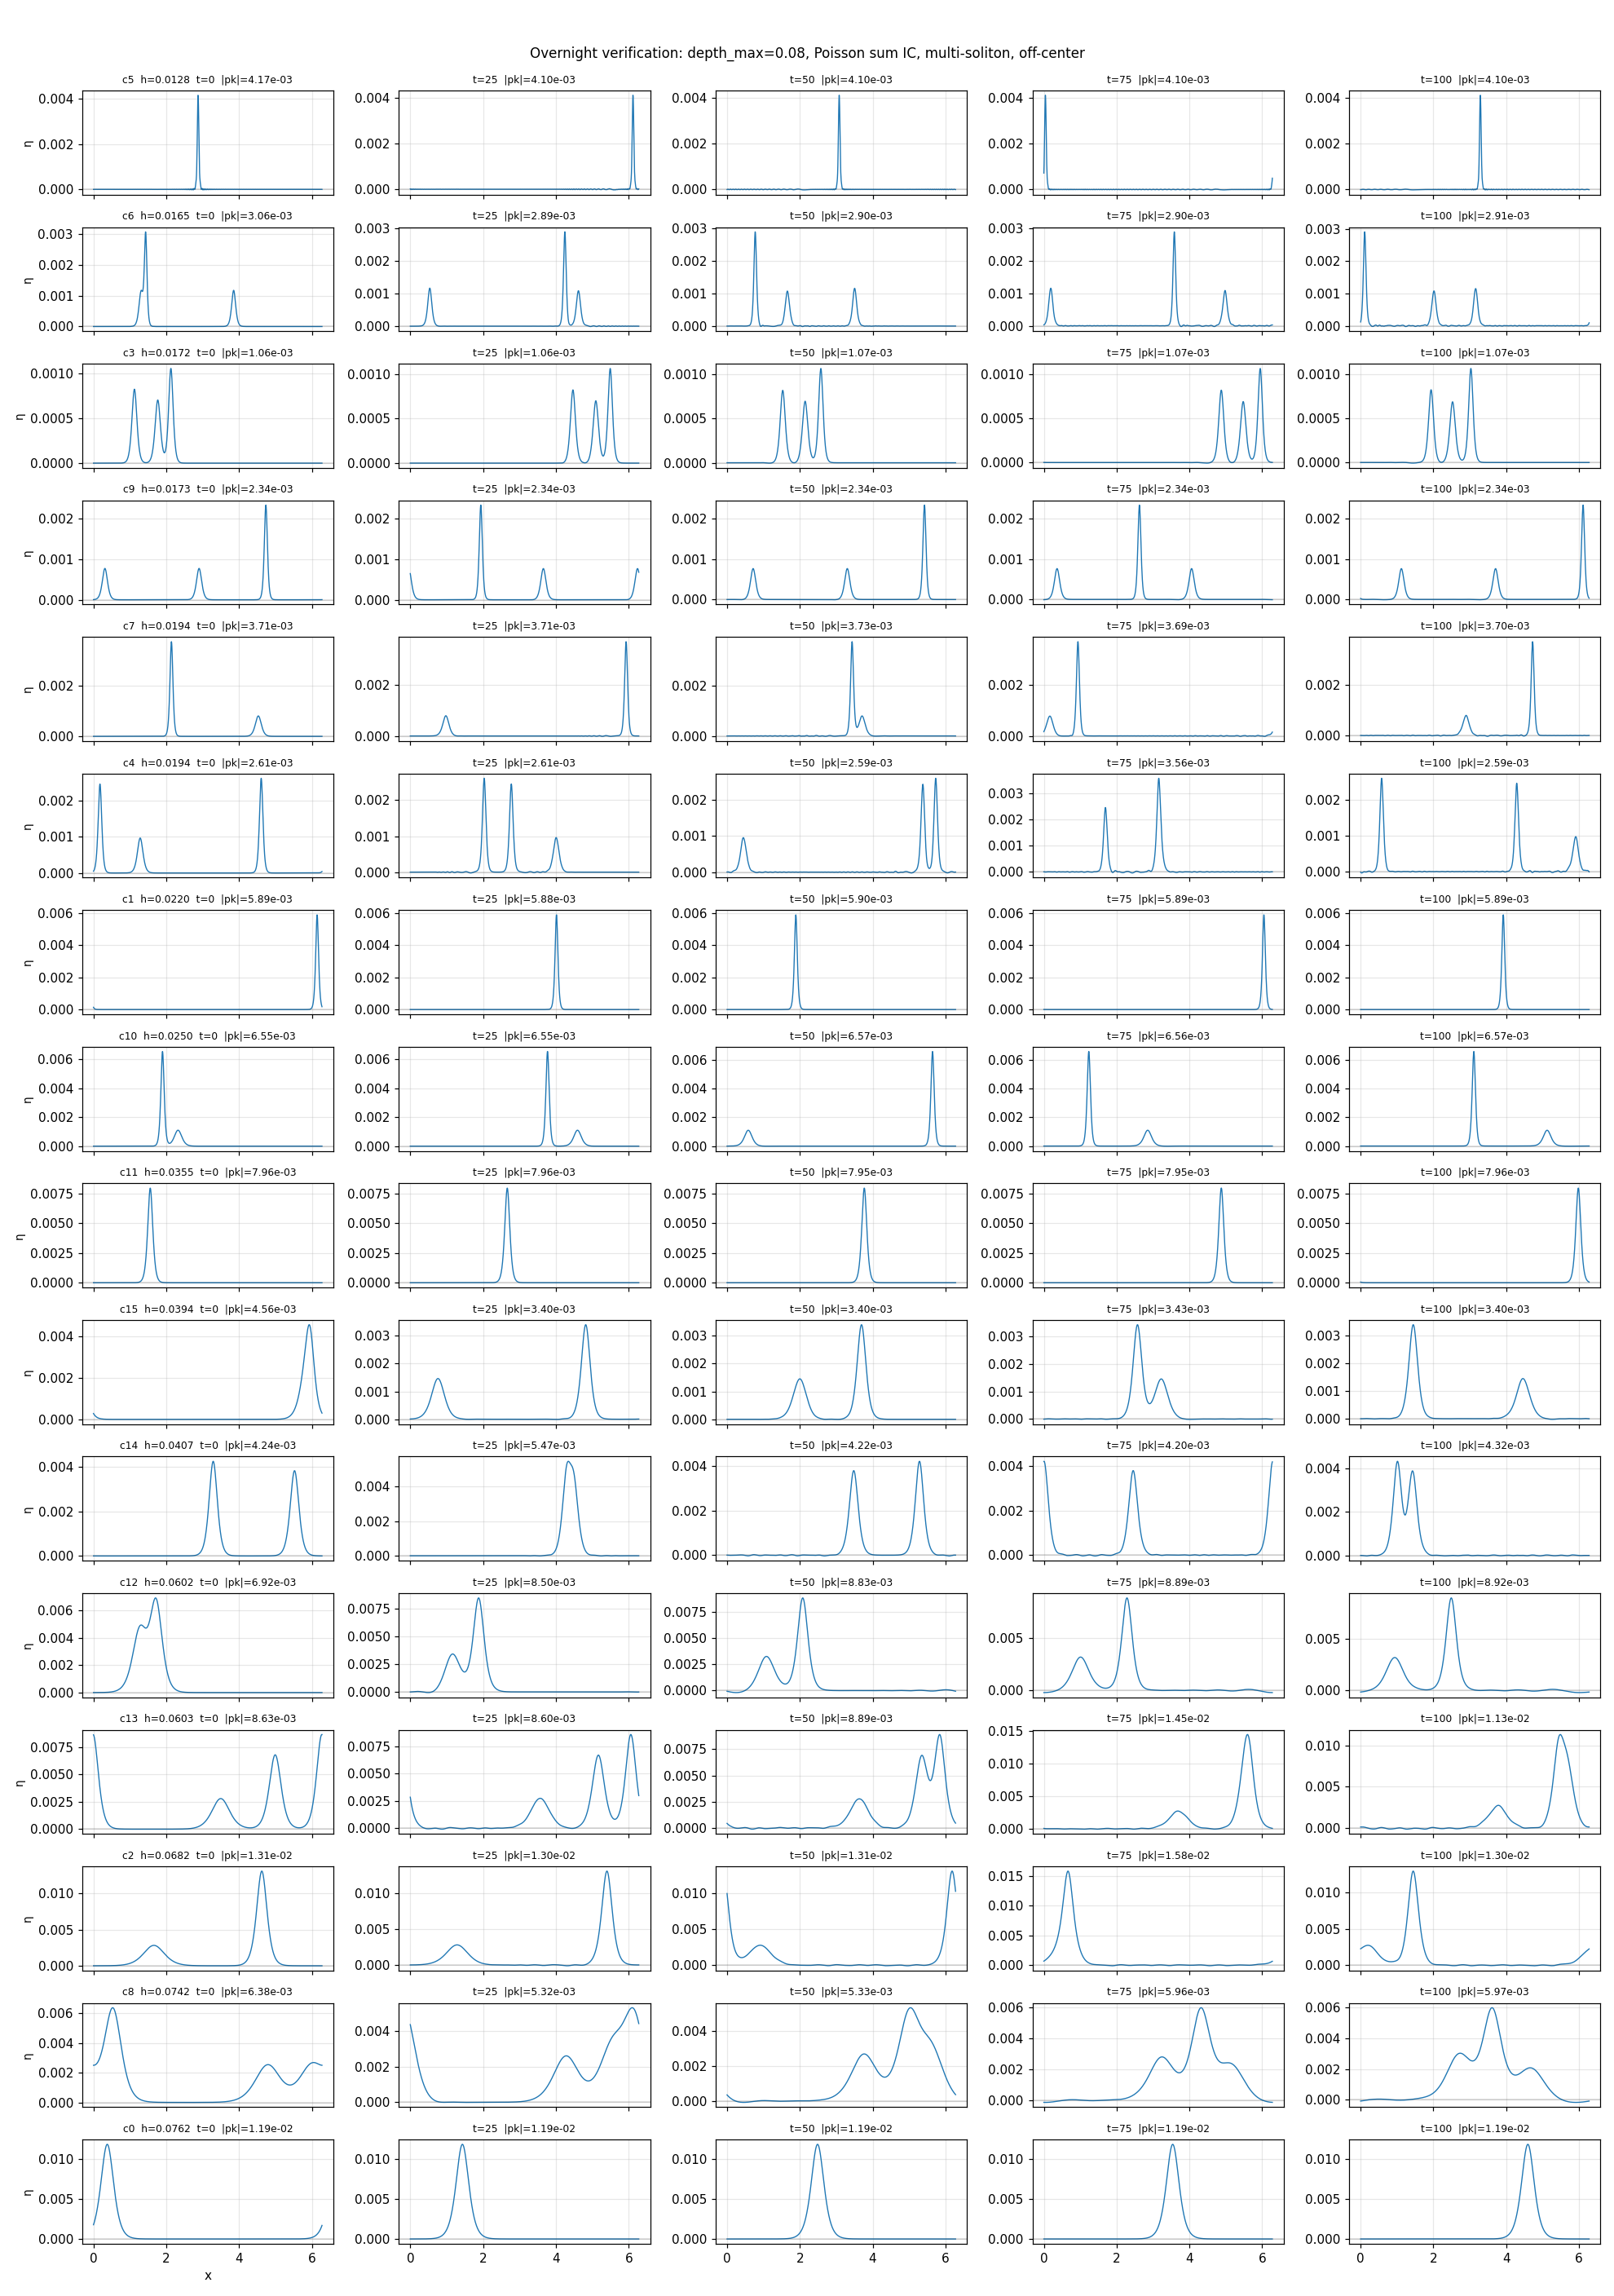
\includegraphics[width=\linewidth]{v2_d008_overnight_rollouts.png}
  \caption{Overnight verification: 16 cases at $h_{\rm ref}$ logUniform on
  $[0.01, 0.08]$ with random multi-crest specs (1--3 solitons per case)
  rolled out to $t = 100$ (the production-settings $t = 200$ rollout is
  qualitatively identical and is summarised in the table above). Rows sorted
  by $h_{\rm ref}$; columns at $t \in \{0, 25, 50, 75, 100\}$. No squiggles.}
  \label{fig:overnight}
\end{figure}

\section{Stress test: where does the new fixed solver actually fail?}

Once the production setting was verified, a stress test mapped the
$(h_{\rm ref}, \alpha)$ grid (where $\alpha = a/h$ is the per-crest steepness)
beyond the production cap to find the failure boundary of the new fixed solver.
Single-soliton single-batch at $t_{\rm max} = 30$, then a follow-up at
$t_{\rm max} = 50$ at the suspected boundary corners.

\subsection{Grid sweep, single soliton, random off-center placement}

\begin{center}
\small
\textbf{Max sign flips on $G\xi$ over $t \in [0, 30]$:}\\[2pt]
\begin{tabular}{c|cccc}
\toprule
$h_{\rm ref} \backslash \alpha$ & $0.10$ & $0.20$ & $0.30$ & $0.40$ \\
\midrule
$0.05$ & 2 & 2 & 2 & 2 \\
$0.10$ & 2 & 2 & 2 & 2 \\
$0.15$ & 2 & 2 & 2 & 2 \\
$0.20$ & 2 & 2 & 2 & 2 \\
$0.25$ & 2 & 2 & 2 & 2 \\
$0.30$ & 4 & 2 & 2 & 2 \\
$0.40$ & 4 & 2 & 2 & 2 \\
\bottomrule
\end{tabular}
\quad
\textbf{$k[80,128)$ growth ratio $t=30 / t=0$:}\\[2pt]
\begin{tabular}{c|cccc}
\toprule
$h_{\rm ref} \backslash \alpha$ & $0.10$ & $0.20$ & $0.30$ & $0.40$ \\
\midrule
$0.05$ & 0.37 & 0.76 & 0.93 & 0.98 \\
$0.10$ & 0.60 & 0.38 & 0.14 & 0.41 \\
$0.15$ & 0.39 & 0.57 & 0.34 & 0.52 \\
$0.20$ & 0.57 & 0.63 & 0.38 & 0.97 \\
$0.25$ & 0.58 & 0.48 & 0.43 & 1.18 \\
$0.30$ & 0.59 & 0.46 & 0.50 & \textbf{2.74} \\
$0.40$ & 0.57 & 0.57 & 0.50 & \textbf{19.25} \\
\bottomrule
\end{tabular}
\end{center}

The sign-flip metric \emph{misses} the failure: counts stay bounded at $2$--$4$
across the whole grid because the contamination is still small in absolute
amplitude at $t = 30$. The band-energy growth ratio reveals a sharp corner at
$(h_{\rm ref} \geq 0.30, \alpha \geq 0.40)$.

\subsection{Borderline cases at longer $t_{\rm max} = 50$}

At the borderline corners, run for longer to see if the growth saturates or
keeps accelerating:

\begin{center}
\begin{tabular}{l c c c c}
\toprule
case & $h_{\rm ref}$ & $\alpha$ & $k[80,128)$ growth $t=50/t=0$ & verdict \\
\midrule
safe   & 0.05 & 0.10 & $0.26\times$         & flat / decay \\
mild   & 0.25 & 0.40 & $1.71\times$         & mild growth \\
border & 0.30 & 0.40 & $\mathbf{26.83\times}$ & accelerating \\
broken & 0.40 & 0.40 & $\mathbf{1186\times}$  & exponential \\
\bottomrule
\end{tabular}
\end{center}

The band-energy growth at the broken corner is exponential in time --- in
$50$ time units it goes from $3 \times 10^{-6}$ to $3.6 \times 10^{-3}$, an
$\sim 1200\times$ increase. Extrapolated to the production $t_{\rm max} = 200$
this would NaN.

\subsection{Multi-crest sweep, $h_{\rm ref} \in \{0.05, 0.10, 0.15, 0.20\}$, sum-budget $\alpha \in [0.30, 0.40]$}

\begin{center}
\begin{tabular}{c|cc}
\toprule
$h_{\rm ref}$ & $n_{\rm crests}=2$ growth & $n_{\rm crests}=3$ growth \\
\midrule
0.05 & $1.10\times$ (max flips $6$) & $0.58\times$ (max flips $8$) \\
0.10 & $0.51\times$ (max flips $4$) & $0.54\times$ (max flips $8$) \\
0.15 & $0.60\times$ (max flips $2$) & $0.63\times$ (max flips $4$) \\
0.20 & $0.54\times$ (max flips $4$) & $0.60\times$ (max flips $4$) \\
\bottomrule
\end{tabular}
\end{center}

Multi-crest at sum-budget steepness up to $\alpha_{\rm sum} = 0.40$ never
shows the boundary growth. The Dirichlet split means no individual crest
reaches $\alpha = 0.40$; the largest crest is typically $\sim 0.25$, well
inside the safe single-soliton corner.

\subsection{Safe envelope}

\begin{itemize}
  \item \textbf{Single soliton}: $h_{\rm ref} \leq 0.25$ at any $\alpha \leq 0.40$;
        or $h_{\rm ref} \leq 0.40$ if $\alpha \leq 0.30$.
  \item \textbf{Multi-soliton (sum-budget)}: $h_{\rm ref} \leq 0.20$ at sum-budget
        $\leq 0.40$ tested clean. (Boundary likely extends further; not pushed.)
  \item \textbf{Production setting} ($\texttt{depth\_max} = 0.08$,
        $\texttt{steepness\_max} = 0.35$, $n_{\rm crests} \in \{1, 2, 3\}$): sits
        $\sim 3\times$ inside the strictest tested bound. Comfortably inside
        the safe interior.
\end{itemize}

\begin{figure}[t]
  \centering
  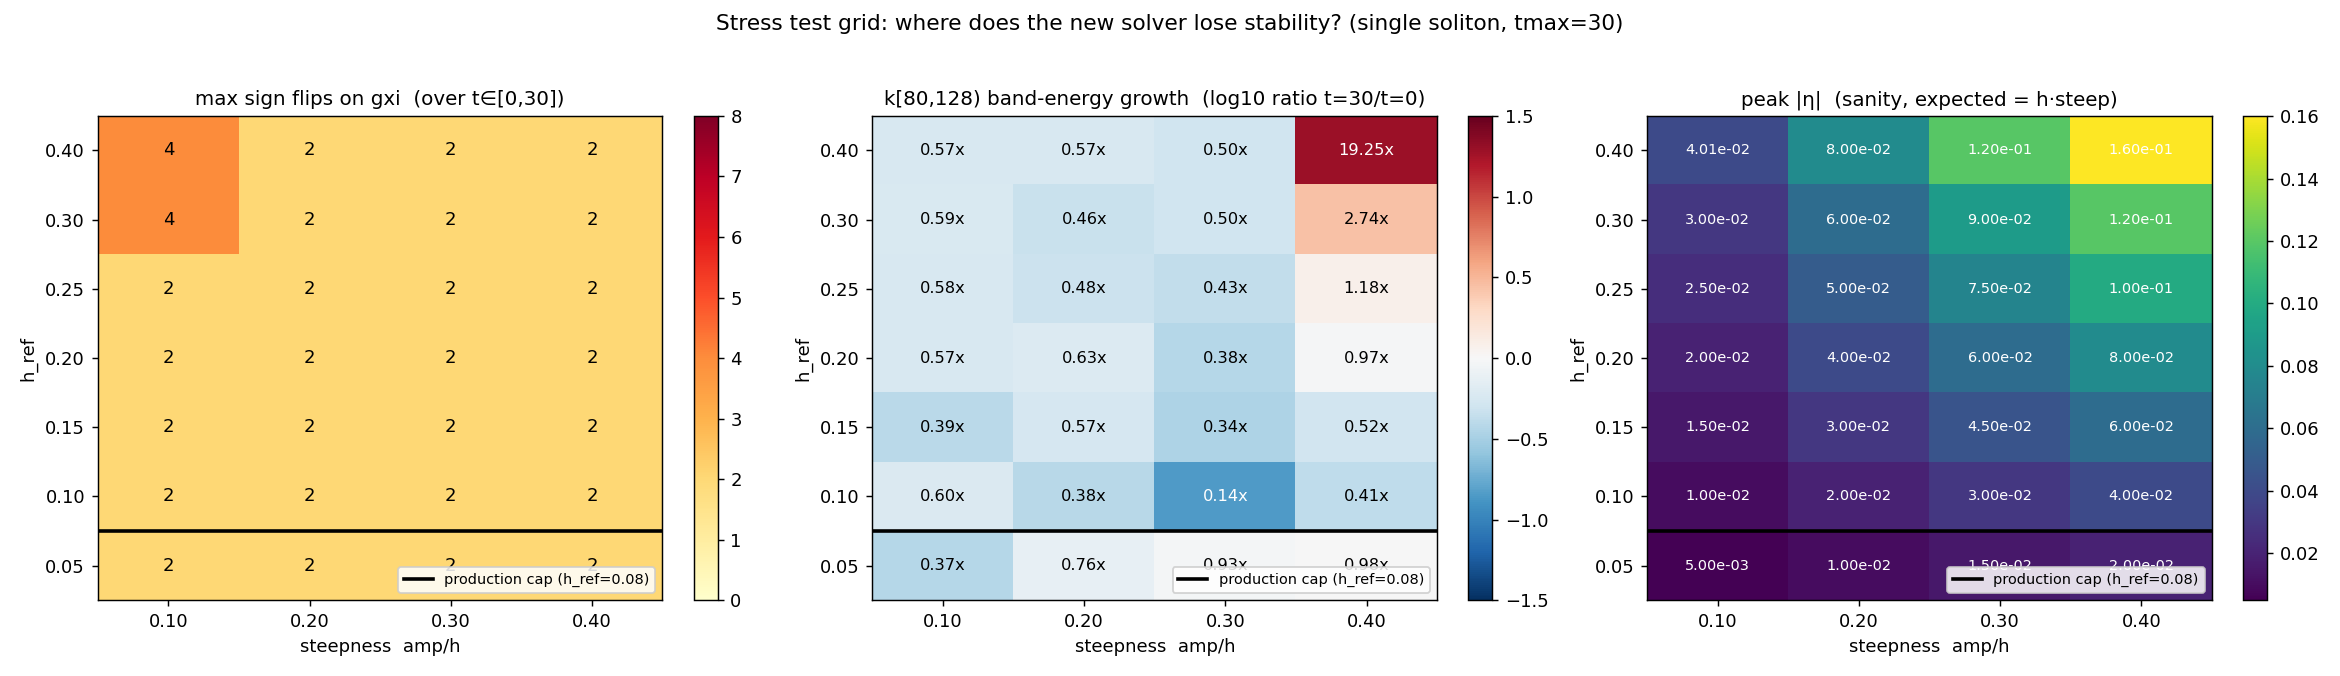
\includegraphics[width=\linewidth]{v2_stress_grid.png}
  \caption{Stress test grid (single soliton, $t_{\rm max} = 30$). Left: max sign
  flips on $G\xi$ (misses the failure). Middle: $\log_{10}$ of the $k[80,128)$
  growth ratio --- the corner $(h_{\rm ref}{=}0.40, \alpha{=}0.40)$ glows red.
  Right: peak $|\eta|$ for sanity, equal to $h_{\rm ref} \cdot \alpha$ as expected.
  Black horizontal line marks the production cap $h_{\rm ref} = 0.08$, which
  sits well inside the safe region.}
  \label{fig:stress-grid}
\end{figure}

\section{Notes for the future}

\begin{itemize}
  \item Tanaka solitons sit at $h \cdot k_{\rm char} \sim \mathcal{O}(1)$ regardless
        of $h_{\rm ref}$, because the soliton width $W \sim h_{\rm ref}$ and so
        $k_{\rm char} \sim 1/W \sim 1/h_{\rm ref}$. This means varying
        $h_{\rm ref}$ on a fixed-$L$ domain does not sweep the dispersive
        regime $h \cdot k_p$ --- it only sweeps the per-soliton domain
        occupancy. To genuinely span shallow-vs-deep water regimes, an IC
        family with a fixed intrinsic scale (random sea state with prescribed
        peak $k_p$, sinusoidal modes, bichromatic packets) is needed; varying
        $h$ then moves the sample across $h \cdot k_p$ regimes.
  \item Spectral filter $\nu = 1/4$ on $L = 2\pi$, $N_x = 1024$ leaves
        $k_{\rm cut} = 128$. The Tanaka soliton's spectrum decays exponentially
        past $k \sim 1/h_{\rm ref}$, so for $h_{\rm ref} \geq 0.01$ the soliton's
        intrinsic content is well below $k_{\rm cut}$. The filter does its job
        of suppressing $k^M$-amplified roundoff without mutilating the
        physical signal.
  \item For any future ICs that involve placing localized profiles on a
        periodic domain, the lesson is: \emph{if the source profile has
        non-zero tails inside the period, use periodic interpolation
        (Poisson summation / wraparound), not zero-extension}. Combining
        \texttt{interp(left=0, right=0)} with random off-center placement
        is a footgun.
\end{itemize}

\end{document}
